\documentclass[aspectratio=169]{beamer}

% Should be first
\usepackage[english]{babel}
\usepackage{fontspec}
\usepackage[utf8]{luainputenc}

% Must be included before tikz when using dvipsnames option (See https://en.wikibooks.org/wiki/LaTeX/Colors#The_68_standard_colors_known_to_dvips)
\usepackage{xcolor}

% No special constraints on order
\usepackage{academicons}
\usepackage[%
        backend=biber,
        safeinputenc,
        sorting=none,
        style=numeric
    ]{biblatex}
\usepackage{calc}
\usepackage{csquotes}
\usepackage{fontawesome}
\usepackage{pgf-umlsd}
\usepackage{minted}
\usepackage{multicol}
\usepackage{nameref}
\usepackage{smartdiagram}
\usepackage{svg}
\usepackage{tikz}
\usepackage[absolute, overlay]{textpos}
\usepackage{xspace}

\usetikzlibrary{calc, positioning}

% Configure minted
\setminted{
    autogobble,
    breaklines=true,
    fontsize=\scriptsize
}

% Animated bubble diagram
\tikzset{%
    Partha/.cd,
    start angle/.initial=0,
    orientation/.initial=1
}
\makeatletter
\newlength{\bubbleInitAngle}
\newcommand{\BubbleDiagramAnimated}[2][]{%
    \begin{tikzpicture}[%
        every node/.style={align=center,let hypenation},
        Partha/.cd,#1
    ]
    \setlength{\bubbleInitAngle}{%
        \ifnumequal{\pgfkeysvalueof{/tikz/Partha/orientation}}{1}{0pt}{-180pt}
    }
    \foreach \smitem [count=\xi] in {#2}{\global\let\maxsmitem\xi}
    \pgfmathtruncatemacro\actualnumitem{\maxsmitem-1}
    \foreach \smitem [count=\xi] in {#2}{%
        \ifnumequal{\xi}{1}{ %true
            \node[bubble center node, smvisible on=<\xi->](center bubble){\smitem};
        }{%false
            \pgfmathtruncatemacro{\xj}{\xi-1}
            \pgfmathtruncatemacro{\angle}{
                \pgfkeysvalueof{/tikz/Partha/start angle}
                + (\pgfkeysvalueof{/tikz/Partha/orientation} * 360 / \actualnumitem * \xj)
                + \bubbleInitAngle
            }
            \edef\col{\@nameuse{color@\xj}}
            \node[bubble node, smvisible on=<\xi->](module\xi) at (center bubble.\angle) {\smitem};
        }%
    }%
    \end{tikzpicture}
}
\makeatother

% Fullscreen frames
\newcommand{\plainFrame}[1]{%
    {
        \setbeamertemplate{headline}{\vskip-\headheight}
        \setbeamertemplate{footline}{\defaultfootline}
        \begin{frame}
            \vspace{-\headheight} % FIXME headline seems not to work as expected
            #1
        \end{frame}
    }
}
\newcommand{\imageFrame}[2][0pt]{%
    {
        \setbeamertemplate{headline}{}
        \setbeamertemplate{footline}{\defaultfootline}
        \begin{frame}
            \begin{textblock*}{\pagewidth} (0pt, #1)
                \centering
                \includegraphics[width=\pagewidth,height=\pageheight,keepaspectratio]{#2}
            \end{textblock*}
        \end{frame}
    }
}
\newcommand{\imageFrameSvg}[1]{%
    {
        \setbeamertemplate{headline}{}
        \setbeamertemplate{footline}{\defaultfootline}
        \begin{frame}
            \begin{textblock*}{\pagewidth} (0pt, 0pt)
                \centering
                \includesvg[width=\textwidth,height=\textheight]{#1}
            \end{textblock*}
        \end{frame}
    }
}
\newcommand{\videoFrame}[2]{%
    {
        \setbeamertemplate{headline}{\vskip-\headheight}
        \setbeamertemplate{footline}{\defaultfootline}
        \begin{frame}
            \centering
            \Huge{\href{run:#1}{#2}}
        \end{frame}
    }
}
\newcommand{\draftFrame}[1]{%
    \begin{frame}[plain]
        \centering
        {\Huge \draft{#1}}
    \end{frame}
}

% Subsection color box
\makeatletter
\newcommand*{\currentname}{\@currentlabelname}
\makeatother

\newcommand<>{\subsectionBox}[1]{%
    \uncover#2{%
        \begin{tikzpicture}[remember picture,overlay]%
            \draw[fill=#1, draw=none]
                (current page.north west) rectangle ++(20pt, -\pageheight);
            \node[anchor=south west] at (current page.south west)
                {\large \rotatebox{90}{\currentname}};
        \end{tikzpicture}
    }
}

% Short codes
\newcommand{\orcid}[1]{\href{https://orcid.org/#1}{\textcolor[HTML]{A6CE39}{\aiOrcid}}}
\newcommand{\drivebuild}{{\scshape DriveBuild}}
\newcommand{\Eg}{E.\,g.\xspace}
\newcommand{\draft}[1]{\color{red} \textit{#1}}
\newcommand{\draftItemize}[1]{%
    \begin{itemize}
        \color{red}
        \itshape{}
        #1
    \end{itemize}
}
\newcommand{\sectionFrame}{%
    \begin{frame}
        \vfill
        \centering
        \begin{beamercolorbox}[sep=8pt,center,shadow=true,rounded=true]{title}
            \usebeamerfont{title}\insertsectionhead\par%
        \end{beamercolorbox}
        \vfill
    \end{frame}
}



\title{DriveBuild}
\subtitle{Automation of Simulation-based Testing\\of Autonomous Vehicles}
\author{\orcid{0000-0002-6780-6055}Stefan Huber} % chktex 8
\institute{University of Passau}
\titlegraphic{
\includegraphics[height=.10\textheight]{media/logoUniPassau.jpg}}
\date{December 19, 2019}

\usetheme{Rochester}
\beamertemplatenavigationsymbolsempty%
\newcommand{\defaultfootline}{%
    \raisebox{5pt}{\makebox[\paperwidth]{\hfill\makebox[10pt]{\scriptsize\insertframenumber}}}
}
\setbeamertemplate{footline}{\defaultfootline}

\addbibresource{biblio.bib}
\nocite{*}
\renewcommand*{\bibfont}{\scriptsize}

\begin{document}
{
    \setbeamertemplate{footline}{}
    \maketitle%
}

\section{Underlying Idea}
% Goals of testers
\begin{frame}{Goals of Testers}
    \centering
    \begin{tikzpicture}
        \node (training) {
\includegraphics[height=.4\pageheight]{media/clip-art-no-workout-today-clipart-1.jpg}};
        \node[below=of training] (temp) {};
        \node[right=of temp] {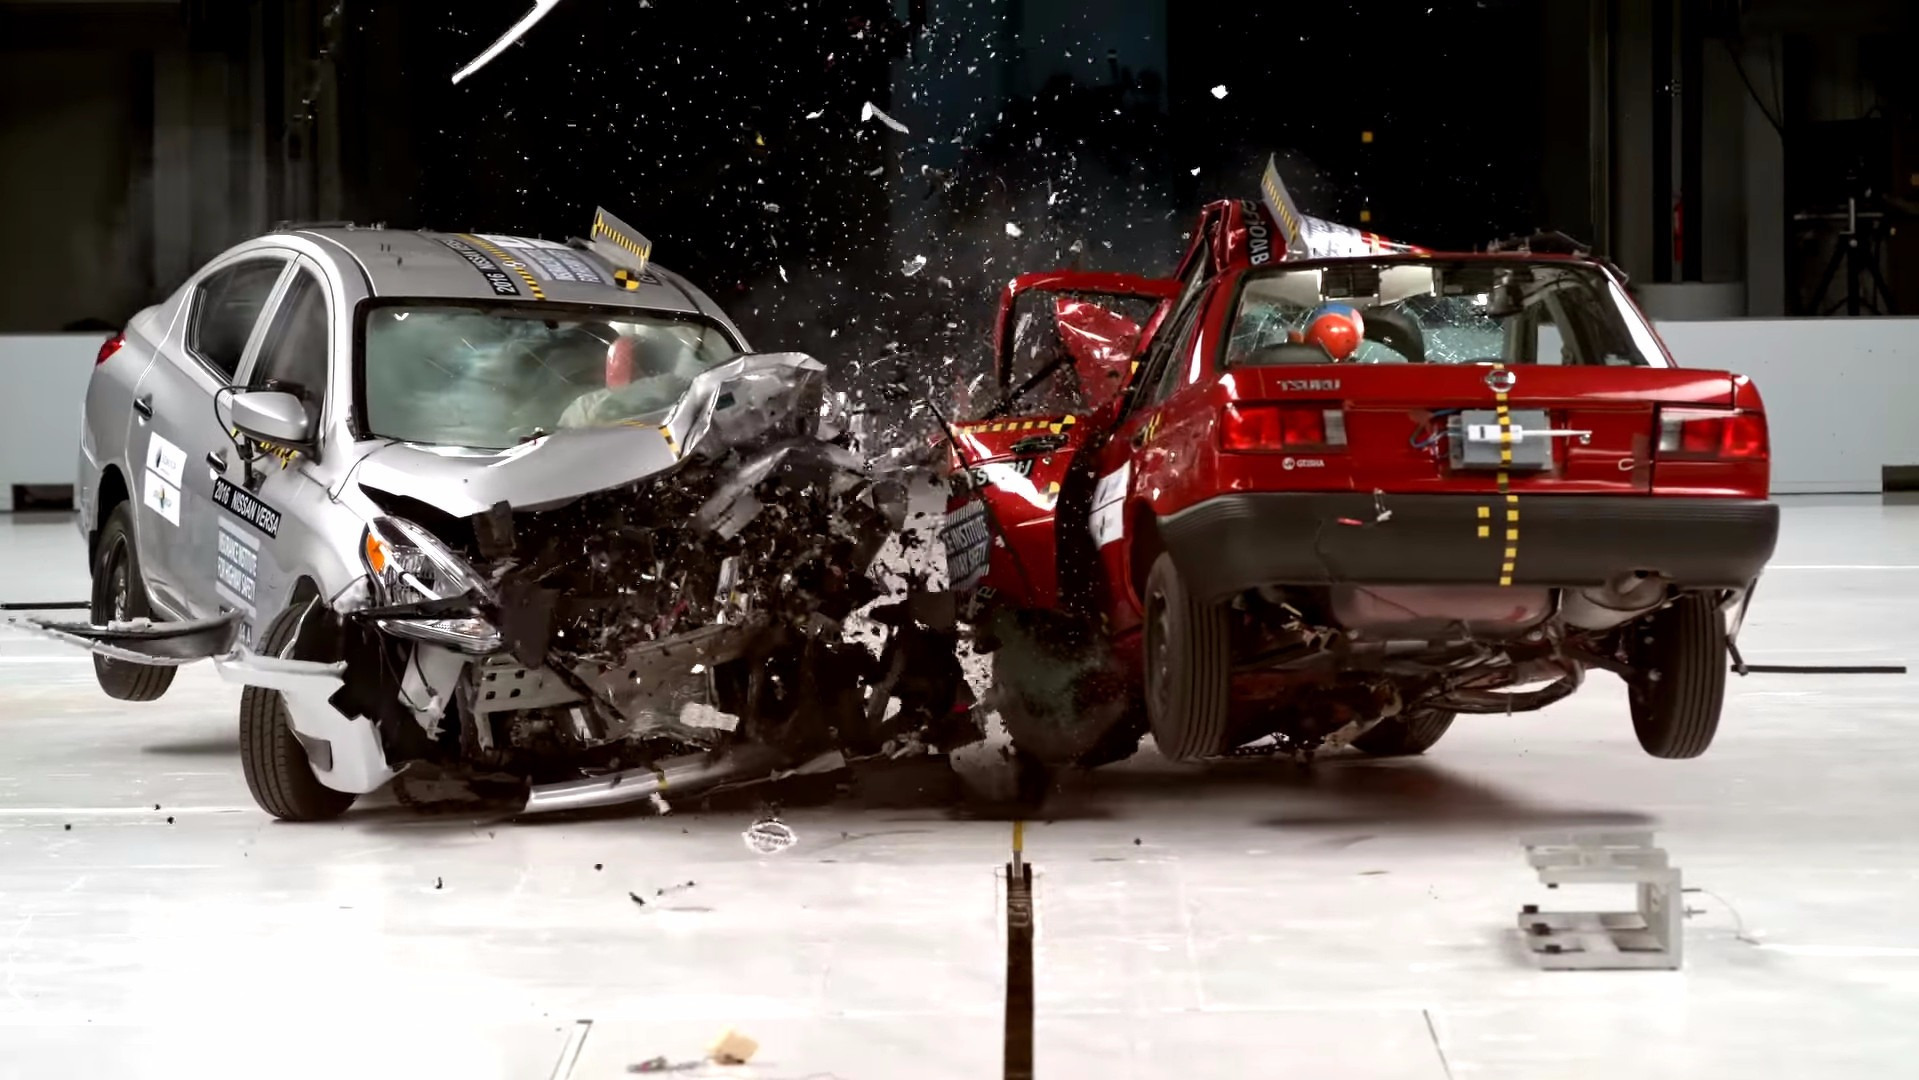
\includegraphics[width=.4\pagewidth]{media/nissan-tsuru-crash-test.jpg}};
        \node[left=of temp] {
\includegraphics[height=.3\pageheight]{media/analyze.png}};
    \end{tikzpicture}
\end{frame}


% Problems testers share
\begin{frame}{Shared Problems}
    \begin{multicols}{2}
        \begin{itemize}[<+ (1)->]
            \item Setup simulator
            \item Distribute and manage test runs
            \item Interact with AIs
            \item Collect data
            \item \(\Rightarrow\) Time consuming
            \item \(\Rightarrow\) Error prone
        \end{itemize}
        \vfill\null%
        \columnbreak%
        \begin{tikzpicture}
            \onslide<2>{\node {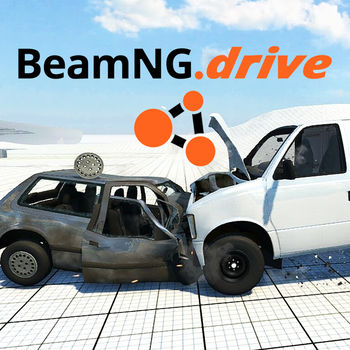
\includegraphics[width=.9\linewidth]{media/beamng-drive-350x350bb}};}
            \onslide<3>{\node {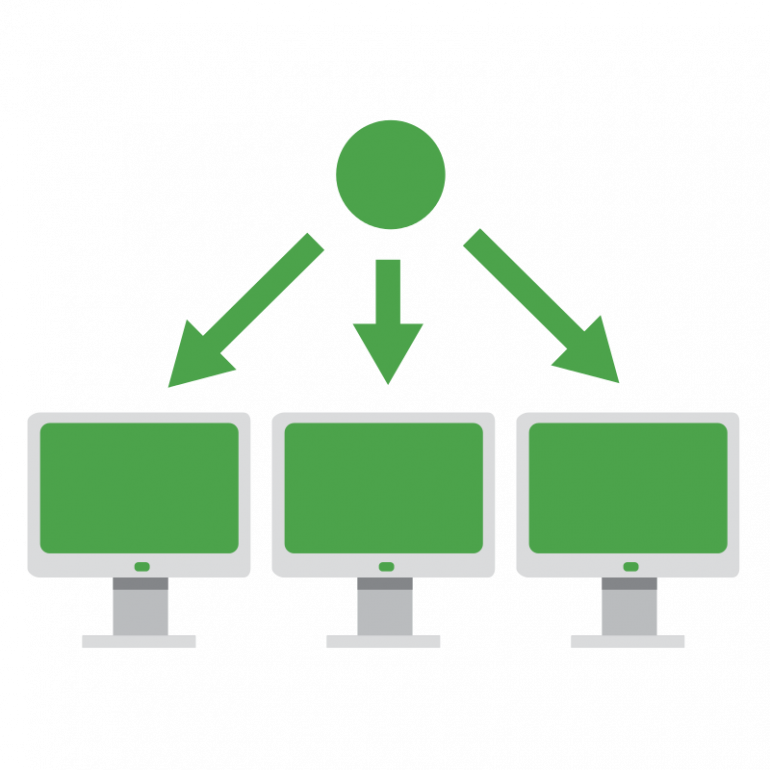
\includegraphics[width=\linewidth]{media/Distributed-770x770.png}};}
            \onslide<4>{\node {
\includegraphics[width=.7\linewidth]{media/img_71102.png}};}
            \onslide<5>{\node {
\includegraphics[width=.8\linewidth]{media/dbms.png}};}
            \onslide<6>{\node {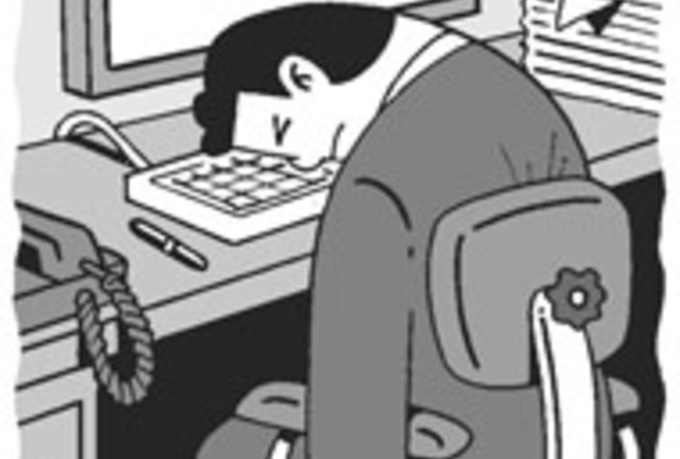
\includegraphics[width=\linewidth]{media/url.jpg}};}
            \onslide<7>{\node {
\includegraphics[width=\linewidth]{media/system-failure.jpg}};}
        \end{tikzpicture}
    \end{multicols}
\end{frame}


\section{Approach of \drivebuild{}}
% Which aspects does DriveBuild handle?
\definecolor{colorFormalize}{HTML}{008148}
\definecolor{colorExecute}{HTML}{C6C013}
\definecolor{colorVerify}{HTML}{EF8A17}
\definecolor{colorGatherData}{HTML}{EF2917}
\plainFrame{%
    \centering
    \smartdiagramset{%
        set color list={colorFormalize,colorExecute,colorVerify,colorGatherData}
    }
    \BubbleDiagramAnimated[%
        orientation=-1
    ]{%
        \drivebuild{},
        Formalization,
        Execution,
        Runtime\\Verification,
        Data\\Collection
    }
    % \smartdiagram[bubble diagram]{%
    %     \drivebuild{},
    %     Formalization,
    %     Execution,
    %     Runtime\\Verification,
    %     Gathering\\Data
    % }
    \smartdiagramset{
        set color list={
            red!40,
            cyan!40,
            blue!40,
            green!40,
            orange!40
        }
    }
}



\subsection{Execution}
% How are tests distributed?
\plainFrame{%
    \centering
    \begin{tikzpicture}[%
            ->,
            >=stealth
        ]
        \node (client) {
\includegraphics[width=.125\linewidth]{media/computer_client.png}};
        \node[right=1.5 of client] (microService) {
\includegraphics[width=.125\linewidth]{media/virtualMachine_microService.png}};
        \draw
            (client) edge (microService)
            (microService) edge (client);
        \node[right=1.5 of microService] (windows2) {
\includegraphics[width=.0625\linewidth]{media/virtualMachine_windows.png}};
        \node[above=0.5 of windows2] (windows1) {
\includegraphics[width=.0625\linewidth]{media/virtualMachine_windows.png}};
        \node[below=0.25 of windows2] (dots) {\vdots};
        \node[below=0.25 of dots] (windows3) {
\includegraphics[width=.0625\linewidth]{media/virtualMachine_windows.png}};
        \draw
            (microService) edge (windows1)
            (windows1) edge (microService)
            (microService) edge (windows2)
            (windows2) edge (microService)
            (microService) edge (windows3)
            (windows3) edge (microService);
        \node[above=of client] (ai1) {
\includegraphics[width=.125\linewidth]{media/img_535483.png}};
        \node[below=of client] (ai2) {
\includegraphics[width=.125\linewidth]{media/img_535483.png}};
        \draw
            (client) edge (ai1)
            (client) edge (ai2);
        \draw
            (ai1) edge (microService)
            (microService) edge (ai1)
            (ai2) edge (microService)
            (microService) edge (ai2);
        \node[right=1.5 of windows2] (dbms) {
\includegraphics[width=.0625\linewidth]{media/dbms.png}};

        \draw
            (dbms) edge (windows1)
            (windows1) edge (dbms)
            (dbms) edge (windows2)
            (windows2) edge (dbms)
            (dbms) edge (windows3)
            (windows3) edge (dbms)
            (microService) edge[bend left=70] (dbms) % FIXME These two edges needed?
            (dbms) edge[bend right=70] (microService);
    \end{tikzpicture}
    \subsectionBox{colorExecute!40}
}



\subsection{Runtime Verification}
% Client side code
%!TEX root = ../2019-12-19_introductionInSeminar.tex
\plainFrame{%
    \centering
    \inputminted{python}{code/manualAi.py}%
    \begin{tikzpicture}[remember picture, overlay]
        \node[anchor=north east] at ($(current page.north east) - (.5, .5)$) {
\includegraphics[width=.1\pagewidth]{media/computer_client.png}};
    \end{tikzpicture}
    \subsectionBox{colorVerify!40}
}


%!TEX root = ../2019-12-19_introductionInSeminar.tex
\plainFrame{%
    \centering
    \inputminted{python}{code/aiStub.py}
    \begin{tikzpicture}[remember picture, overlay]%
        \node[anchor=north east] at ($(current page.north east) - (.5, .5)$) {
\includegraphics[width=.1\pagewidth]{media/img_535483.png}};
    \end{tikzpicture}
    \subsectionBox{colorVerify!40}
}



%!TEX root = ../2019-12-19_introductionInSeminar.tex
\plainFrame{%
    \centering
    \href{https://trackersb.github.io/DriveBuild/}{{\Huge Examples and stubs \faExternalLink}\\{\Large (https://trackersb.github.io/DriveBuild/)}}
}



\section{Installation}
\sectionFrame{}

% \section{Sources}
% \sectionFrame{}
% \begin{frame}[allowframebreaks]{Sources}
%     \printbibliography%
% \end{frame}

\section{Backup Slides}
\sectionFrame{}

\subsection{Formalization}
% What can be formalized?
\plainFrame{%
    \begin{multicols}{2}
        \centering
        {\Large Environment}
        \begin{tikzpicture}
            \pause
            \node (roads) {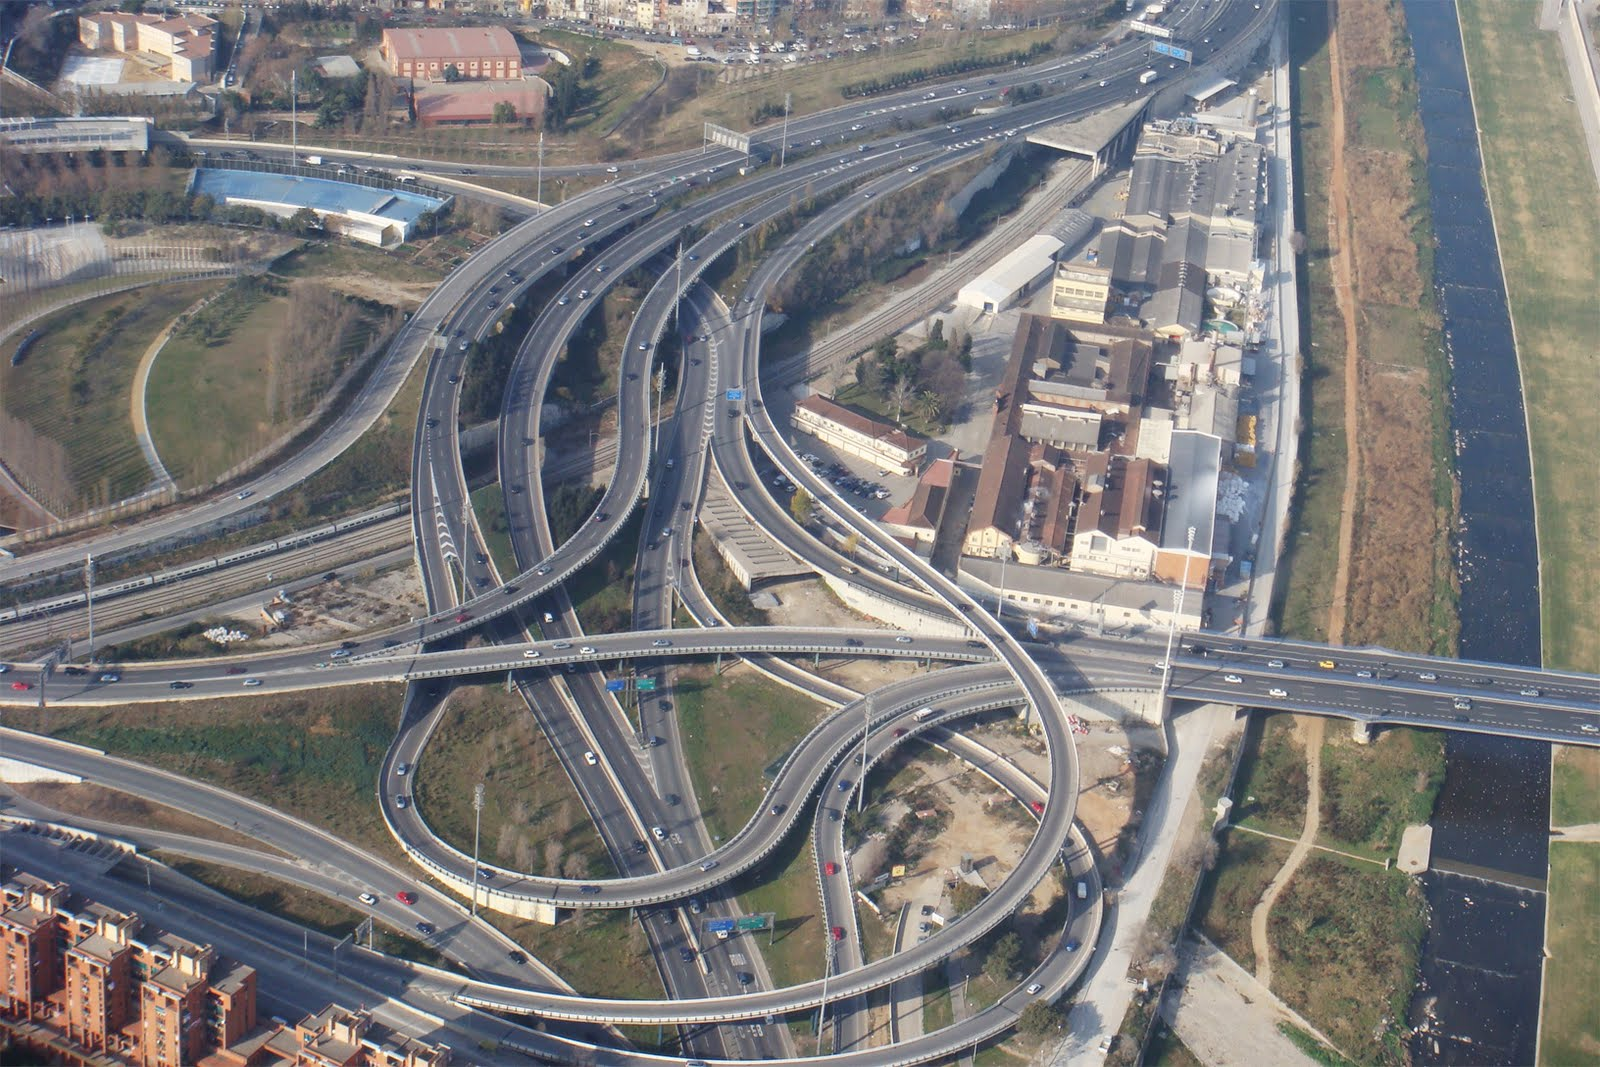
\includegraphics[width=\linewidth]{media/Crazy_Road_Network.jpg}};
            \pause
            \node (obstacles) at (roads.south) {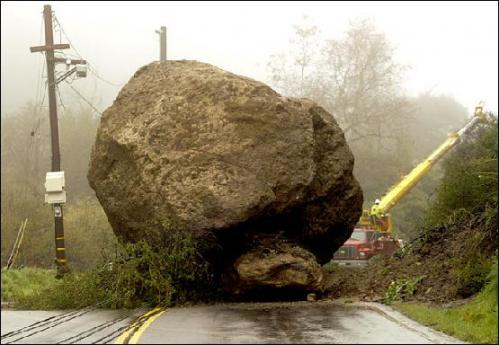
\includegraphics[width=\linewidth]{media/obstacle-on-your-road.jpg}};
        \end{tikzpicture}
        \vfill\null%
        \columnbreak%
        \onslide<1->{{\Large Test Setup}}
        \onslide<4->{
            \begin{tikzpicture}
                \pause
                \node (car) {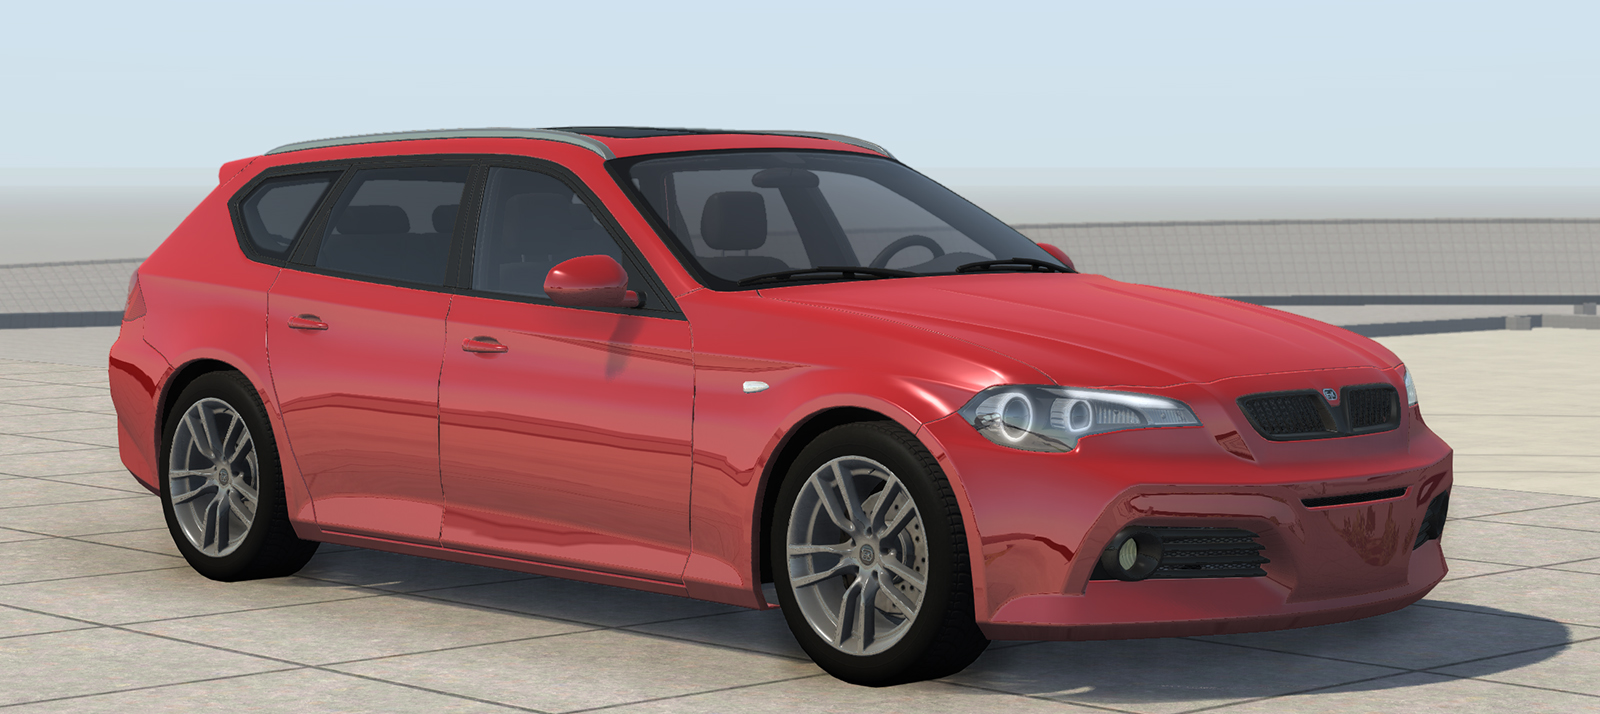
\includegraphics[width=\linewidth]{media/etk800thread.jpg}};
                \pause
                % FIXME Should I mention movement?
                \node (movement) at (car.south) {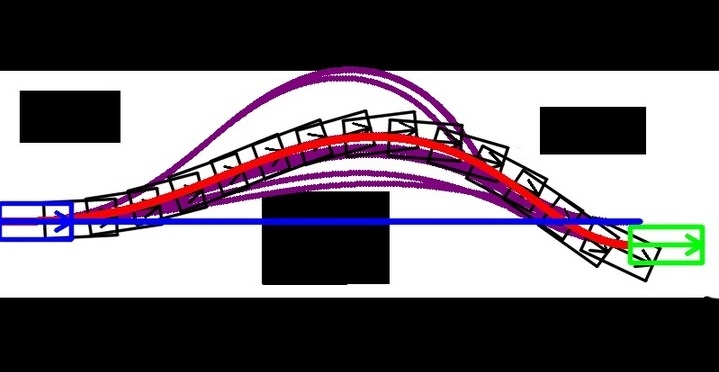
\includegraphics[width=\linewidth]{media/nlp.jpg}};
                \pause
                \node (criteria) at (movement.south) {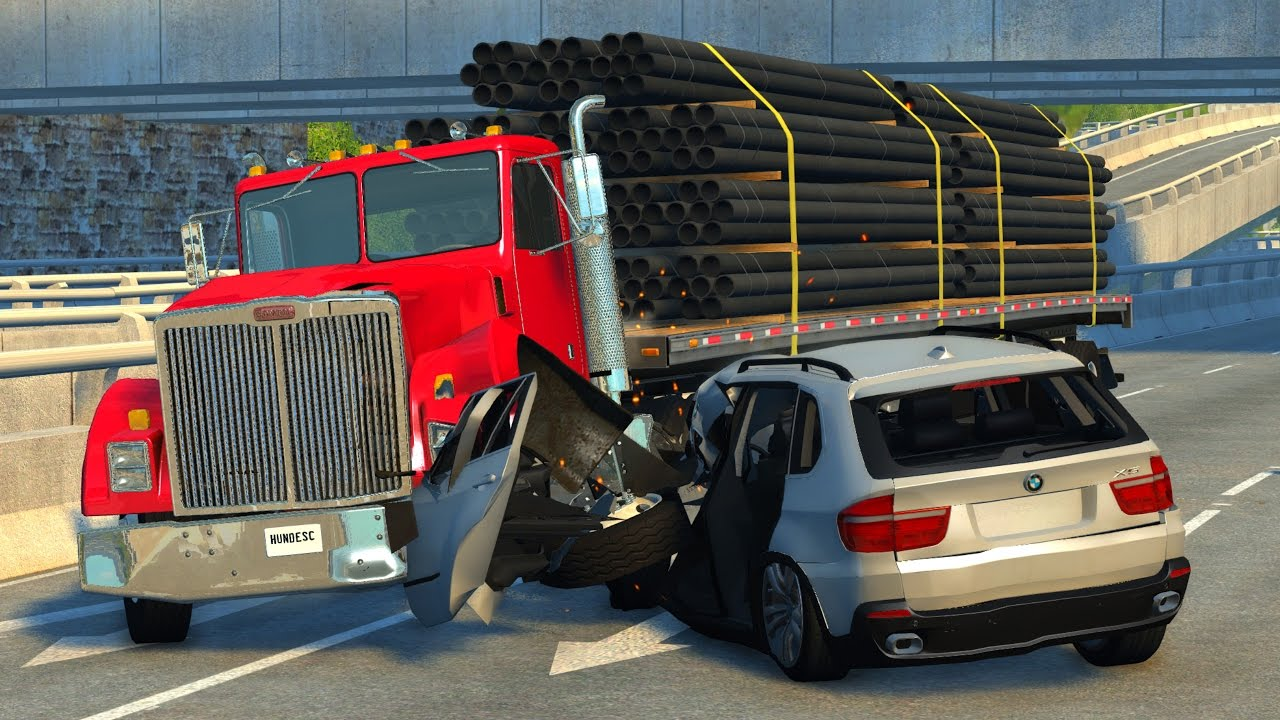
\includegraphics[width=\linewidth]{media/maxresdefault.jpg}};
                \pause
                \node (offroad) at (car) {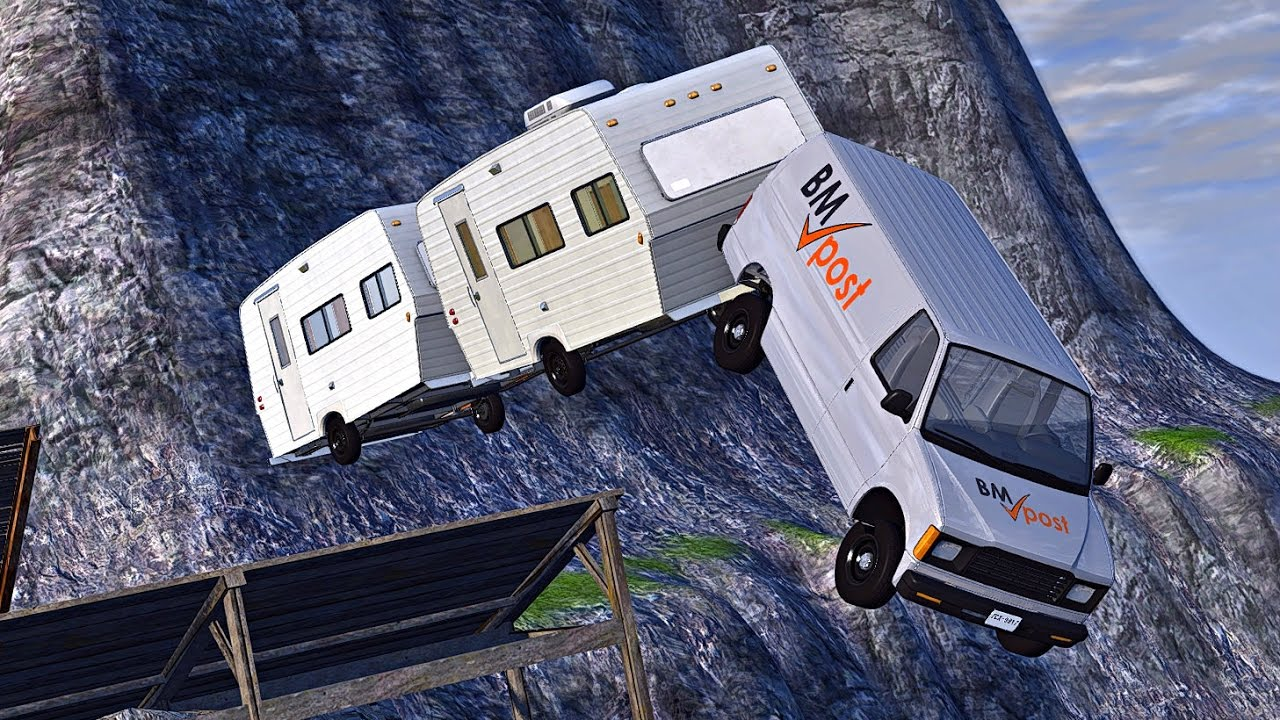
\includegraphics[width=\linewidth]{media/maxresdefault2.jpg}};
                \pause
                \node (finish) at (offroad.south) {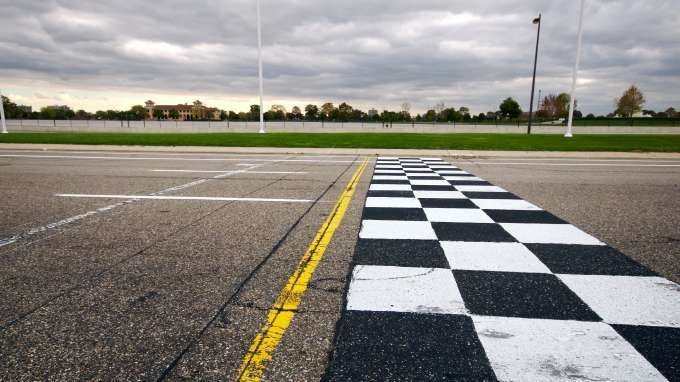
\includegraphics[width=\linewidth]{media/1349.jpg}};
            \end{tikzpicture}
        }
    \end{multicols}
    \subsectionBox<1->{colorFormalize!50}
}



\subsection{Runtime Verification}
% How does the client scheme look like?
\plainFrame{%
    \centering
    \resizebox{!}{\pageheight}{%
        \begin{sequencediagram}
            \newthread{client}{:Client}
            \tikzstyle{inststyle}+=[below right=-0.82cm and 5cm of client]
            \newthread{drivebuild}{:MainApp}
            \begin{call}{client}{/runTests}{drivebuild}{SubmissionResult}
            \end{call}
            \begin{sdblock}{Handle AI}{For each AI in parallel}
                \begin{call}{client}{/ai/waitForSimulatorRequest}{drivebuild}{SimStateResponse}
                    \begin{callself}{drivebuild}{Wait for requestAiFor}{}
                    \end{callself}
                \end{call}
                \begin{call}{client}{/ai/requestData}{drivebuild}{DataResponse}
                \end{call}
                \begin{callself}{client}{Calculate control commands}{}
                \end{callself}
                \begin{call}{client}{/ai/control}{drivebuild}{Void}
                    \begin{callself}{drivebuild}{Apply control commands}{}
                    \end{callself}
                \end{call}
            \end{sdblock}
        \end{sequencediagram}
    }
    \subsectionBox{colorVerify!40}
}



% What steps does the runtime verification?
\plainFrame{%
    \centering
    \smartdiagram[circular diagram:clockwise]{%
        Verify criteria, Request AIs, Control, Step, Pause
    }
    \subsectionBox<1->{colorVerify!40}
}



\subsection{Data Collection}
% Which data is available?
\newlength{\imageWidth}
\setlength{\imageWidth}{.33\textwidth}
\newlength{\imageHeight}
\setlength{\imageHeight}{.5\textheight}
\plainFrame{%
    \centering
    \subsectionBox<1->{colorGatherData!40}
    
\includegraphics[width=\imageWidth,height=\imageHeight,keepaspectratio]
        {media/location_marker_gps_shutterstock.jpg}
    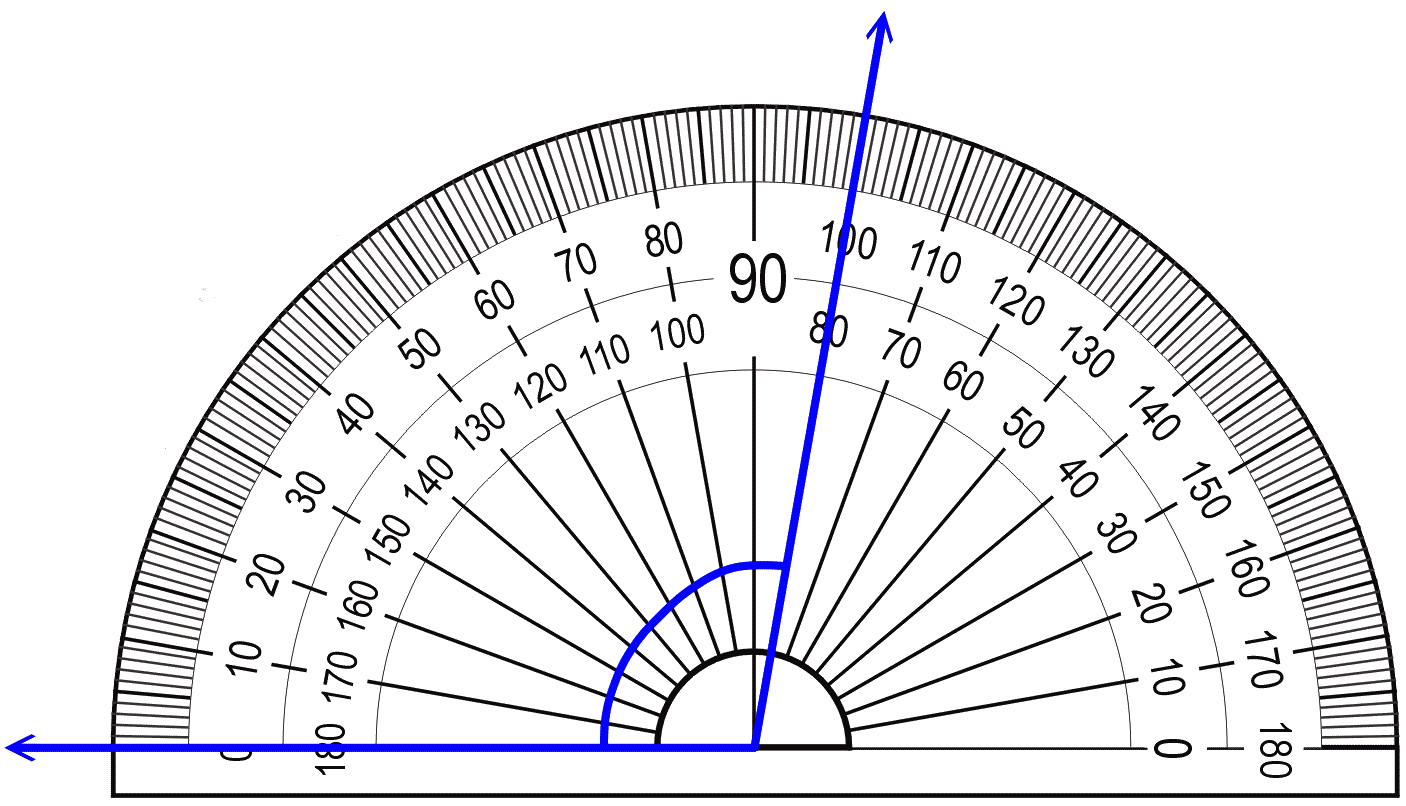
\includegraphics[width=\imageWidth,height=\imageHeight,keepaspectratio]
        {media/measure-angle7.png}
    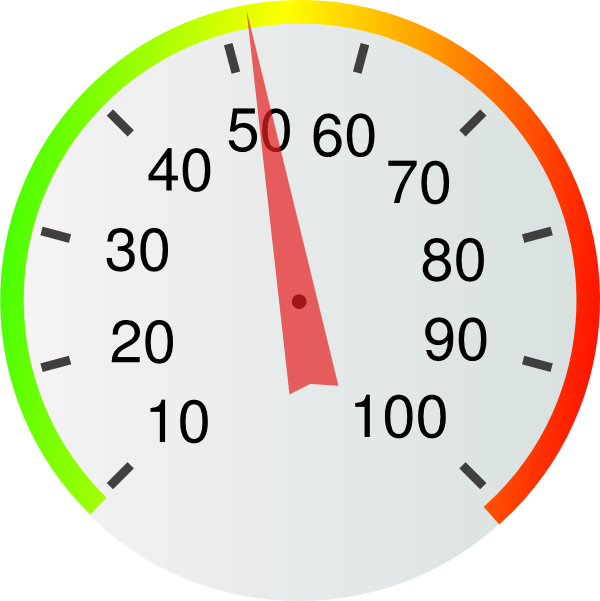
\includegraphics[width=\imageWidth,height=\imageHeight,keepaspectratio]
        {media/tacho-clipart-13.png}
    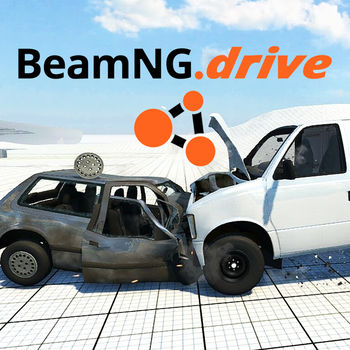
\includegraphics[width=\imageWidth,height=\imageHeight,keepaspectratio]
        {media/beamng-drive-350x350bb.jpg} % chktex 29
    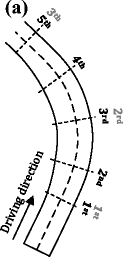
\includegraphics[width=\imageWidth,height=\imageHeight,keepaspectratio]
        {media/12544_2018_284_Fig1_HTML.png}
    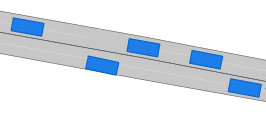
\includegraphics[width=\imageWidth,height=\imageHeight,keepaspectratio]
        {media/DEU_Muc-2_1_T-1.png}
}


\end{document}
